\subsection{Pravljenje naloga klijenta}

Na slici \ref{fig:SignUp} je prikazana stranica za pravljenje naloga klijenta na ChooseFresh sistem. Pored potrebnih podataka, postoji i opcija navigacije ka stranici za prijavljivanje ukoliko je klijent već registrovan. Klijent može proveriti unos u polje \textit{Password} klikom na ikonicu u desnom uglu polja. Takođe, klijent može odabrati opciju da se, nakon registracije, klijent prijavi i ne odjavi sa sistema, sve dok se klijent eksplicitno ne odjavi sa sistema.

\begin{figure}[H]
	\begin{center}
		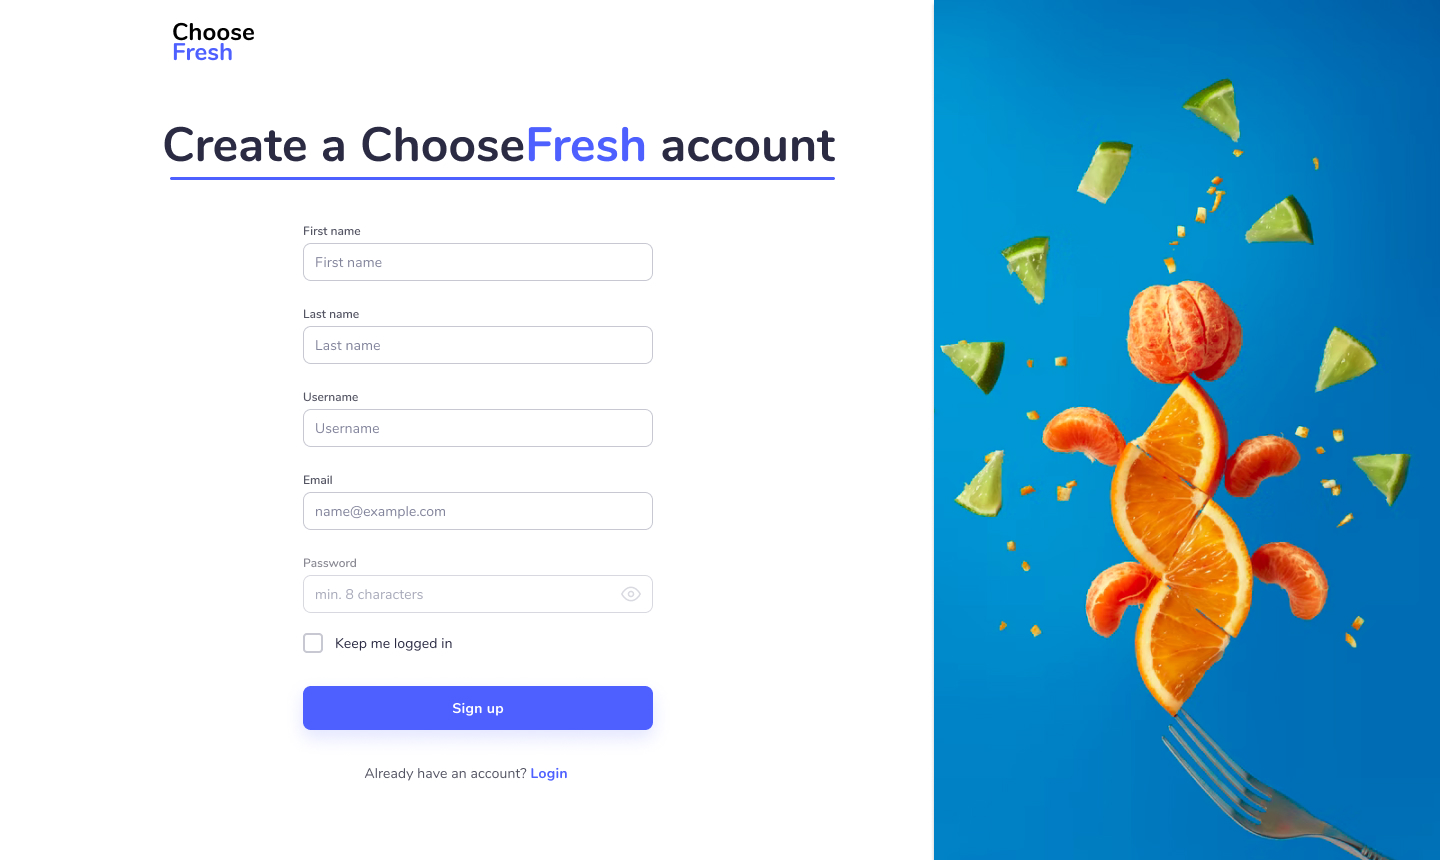
\includegraphics[width=\textwidth]{UI/SignUp.jpg}
    		\caption{Stranica registracije klijenta}
    \label{fig:SignUp}
    \end{center}
\end{figure}


U slučaju da je klijent uneo korisničko ime koje već postoji u sistemu prikazuje se stranica \ref{fig:UsernameExists}, a ukoliko je uneo prekratku šifru, prikazuje se stranica \ref{fig:ShortPassword}  

\begin{figure}[H]
	\begin{center}
		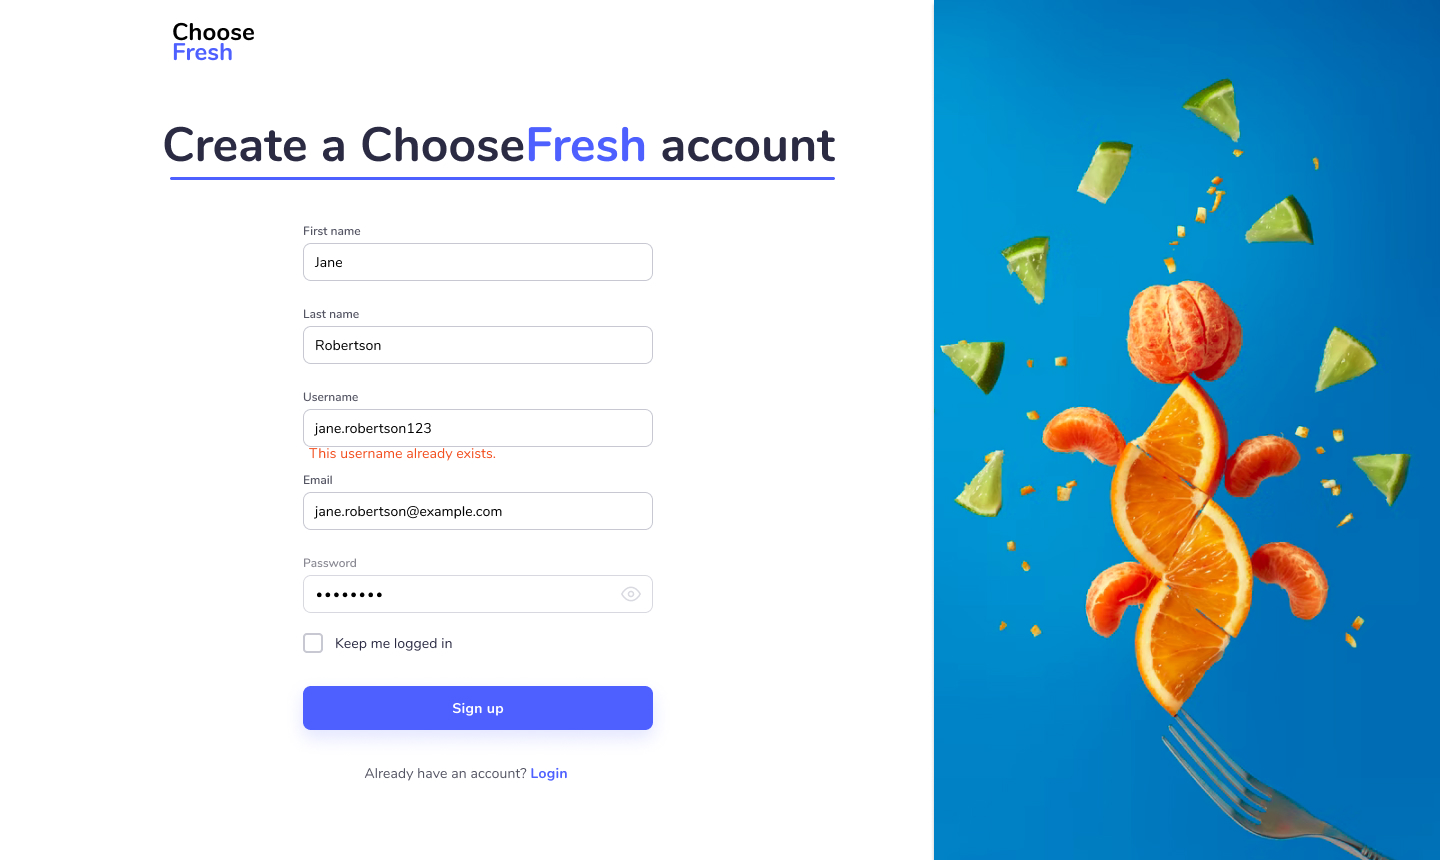
\includegraphics[width=\textwidth]{UI/UsernameExistsSignUp.jpg}
    		\caption{Stranica registracije klijenta ukoliko je korisnik uneo postojeće korisničko ime}
    \label{fig:UsernameExists}
    \end{center}
\end{figure}

\begin{figure}[H]
	\begin{center}
		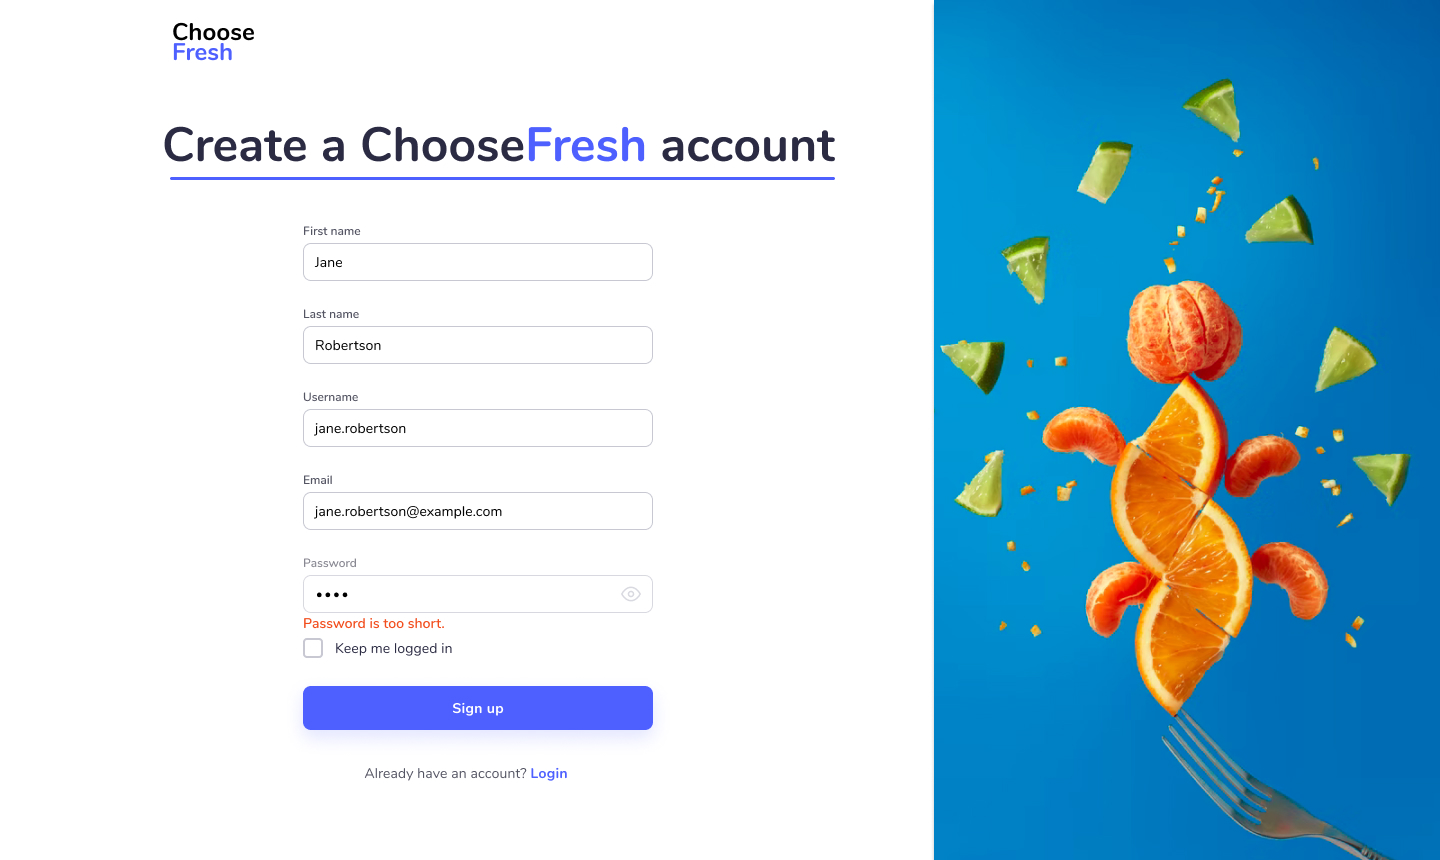
\includegraphics[width=\textwidth]{UI/ShortPasswordSignUp.jpg}
    		\caption{Stranica registracije klijenta ukoliko je korisnik uneo prekratku šifru}
    \label{fig:ShortPassword}
    \end{center}
\end{figure}
